%!TEX TS-program = xelatex
\documentclass[]{friggeri-cv}
\usepackage{afterpage}
\usepackage{hyperref}
\usepackage{color}
\usepackage{xcolor}
\hypersetup{
    pdftitle={},
    pdfauthor={},
    pdfsubject={},
    pdfkeywords={},
    colorlinks=false,       % no lik border color
   allbordercolors=white    % white border color for all
}
\addbibresource{bibliography.bib}
\RequirePackage{xcolor}
\definecolor{pblue}{HTML}{0395DE}

\begin{document}
\header{Daniel}{Pavez-Sandoval}
      {Mag{\'i}ster en Ingenier{\'i}a Inform{\'a}tica}

% Fake text to add separator      
\fcolorbox{white}{gray}{\parbox{\dimexpr\textwidth-2\fboxsep-2\fboxrule}{%
.....
}}

% In the aside, each new line forces a line break
\begin{aside}
    ~
    ~
    ~
    ~
    ~
  \section{Direcci{\'o}n}
    Mar{\'i}n, 0193, 
    Depto. 423
    Providencia, Stgo.
    C{\'o}d. Post.,
    7501353
    ~
  \section{Tel \& Skype}
    +56 9 8943 4150
    daniel.pavez.s
    ~
  \section{Mail}
    \href{mailto:daniel.pavez@usach.cl}{daniel.pavez@ usach.cl}
    \href{mailto:daniel.pavez.s@gmail.com}{daniel.pavez.s@ gmail.com}
    ~
  \section{Web \& Git}
    %\href{https://cl.linkedin.com/in/daniel-ignacio-pavez-sandoval-12297928}{LinkedIn}
    \href{https://cl.linkedin.com/in/daniel-ignacio-pavez-sandoval-12297928}{12297928 (LinkedIn)}
%    \href{https://bitbucket.org/neoben}{bitbucket.org/neoben}
    \href{https://github.com/MnKGuitarPro}{MnKGuitarPro (github)}
    ~
  \section{Programaci{\'o}n}
    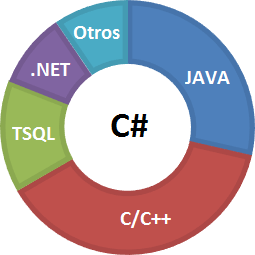
\includegraphics[scale=0.53]{img/Lenguajes.png}
    ~
  \section{Preferencia de OS}
    \textbf{GNU/Linux}
\includegraphics[scale=0.40]{img/5stars.png}
    \textbf{Windows}
\includegraphics[scale=0.40]{img/5stars.png}
    \textbf{Unix}
\includegraphics[scale=0.40]{img/2stars.png}
    \textbf{MacOS}
\includegraphics[scale=0.40]{img/1stars.png}
\end{aside}

\section{Experiencia}
\begin{entrylist}
    \entry
    {01/14 - Ahora}
    {Ingeniero TI \& DBA}
    {Electrolux Chile}
    {Face inicial como Ingeniero TI para soporte de aplicaci{\'o}n orientada a procesos de posventa a nivel internacional, para luego tomar el cargo de administrador y DBA de la mencionada aplicaci{\'o}n, dando soporte a 22 pa{\'i}ses. Posteriormente se toma un cargo como jefe de proyecto para sistema de administraci{\'o}n de conocimiento. Las actividades actuales hacen relaci{\'o}n con gesti{\'o}n documental y m{\'o}dulo PI en ERP SAP.\\}
    \entry
    {06/09 - 12/13}
    {Profesor de Laboratorio}
    {Universidad de Santiago de Chile}
    {Cursos de laboratorio para asignaturas de Organizaci{\'o}n de Computadores; Estructura de Computadores; Sistemas Distribuidos; Taller de Sistemas Distribuidos; Introducci{\'o}n y Fundamentos de Programaci{\'o}n y Bioinform{\'a}tica.\\}    
    \entry
    {10/09 - 10/13}
    {Participante y Entrenador, ACM ICPC}
    {Universidad de Santiago de Chile}
    {Participaci{\'o}n como representante de Universidad de Santiago de Chile en compentencia de programaci{\'o}n {\'a}gil ACM ICPC. A{\~n}o 2009 y 2010 como participante (quinto lugar nacional en a{\~n}o 2010). A{\~n}o 2011 y 2013 como entrenador de equipo que representaba a la Universidad de Santiago de Chile.\\}
    \entry
    {11/10 - 04/11}
    {Desarrollador y dise{\~n}ador Web}
    {DIRECTLink E.I.R.L., Santiago, Chile}
    {Desarrollo de ERP orientado al negocio odontol{\'o}gico: Captura de reque-rimientos, dise{\~n}o de vistas (Web con HTML \& ASP), controlador (C\# \& IIS) y modelo (SQL Server 2008, \textit{Store Procedure}, \textit{function}, \textit{views}, etc.). Configuración de equipos y red \textit{Intranet} para montado de aplicaci{\'o}n Web. Asesor{\'i}a para mejora de proceso de negocio.}
\end{entrylist}

\section{Educaci{\'o}n}
\begin{entrylist}
  \entry
    {2006 - 2013}
    {Grado de Mag{\'i}ster en Ingenier{\'i}a Inform{\'a}tica}
    {Universidad de Santiago de Chile}
    {T{\'o}picos principales:\\ Conceptos avanzados de miner{\'i}a de datos, procesos de negocio, \textit{business intelligence}, bases de datos avanzadas e investigaci{\'o}n.\\
    \emph{T{\'i}tulo de la tesis: ``Incorporaci{\'o}n de Anotaciones G{\'e}nicas en el Algoritmo de Agrupamiento \textit{MST-kNN}''.}\\
    \emph{Profesor gu{\'ia}: Dr. Mario Inostroza-Ponta.}\\}
  \entry
    {2006 - 2013}
    {Ingeniero Civil Inform{\'a}tico}
    {Universidad de Santiago de Chile}
    {T{\'o}picos principales:\\ Conceptos avanzados de programaci{\'o}n (estructuras de datos, paradigmas de programaci{\'o}n, algoritmos y optimizaci{\'o}n), conceptos de sistemas operativos, \textit{hardware}, redes y seguridad. Elementos avanzados de computación paralela, sistemas distribu{\'i}dos, y proyectos de ingenier{\'i}a de \textit{software} y base de datos.\\}
    %\emph{Thesis activity carried out during an internship period at Atitlan Engineering SRL.}\\}
  \entry
    {2006 - 2010}
    {Licenciado en Ciencias de la Computaci{\'o}n}
    {Universidad de Santiago de Chile}
    {T{\'o}picos principales:\\
    Ciencias b{\'a}sicas, matem{\'a}tica avanzada, conceptos elementales de economía, inform{\'a}tica y programaci{\'o}n, e idiomas.}
\end{entrylist}

%\section{Certificaciones}
%\begin{entrylist}
%  \entry
%    {02/2013}
%    {Intro to Computer Science}
%    {Udacity. E-learning}
%    {\emph{Building a Python Search Engine}}
%\end{entrylist}

\newpage

\begin{aside}
    ~
    ~
    ~
  \section{Habilidades Personales}
    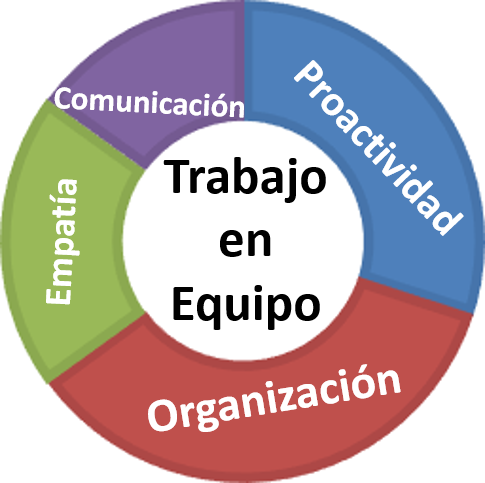
\includegraphics[scale=0.29]{img/Skills4.png}
    ~
  \section{Idiomas}
    \textbf{Espa{\~n}ol}
\includegraphics[scale=0.40]{img/5stars.png}
    \textbf{Inglés}
\includegraphics[scale=0.40]{img/3stars.png}
\end{aside}

\section{Publicaciones}
D. Pavez Sandoval\\
\href{http://jcc2013.inf.uct.cl/wp-content/proceedings/ET/Incorporacion\%20de\%20Anotaciones\%20Geneticas\%20en\%20el\%20Algoritmo\%20de\%20Agrupamiento\%20MST-kNN.pdf}{\textbf{Incorporaci{\'o}n de Anotaciones Gen{\'e}ticas en el Algoritmo de Agrupamiento MST-kNN}}
\emph{Jornadas Chilenas de la Computaci{\'o}n (JCC 2013), Temuco, Chile, Noviembre 11-15, 2013}
\\
\section{Otra informaci{\'o}n}
Para el mercado de trabajo chileno:\\
\emph{Desde corta edad fui atraído por temas relacionados a tecnología e informática, por lo que decidir que carrera profesional seguir, en mi caso, fue fácil. La experiencia y la formación que me entregó la Universidad marcaron mi forma de desenvolverme en el área, y así ha sido hasta el día de hoy. Laboralmente, he trabajado en proyectos de desarrollo de software, como ingeniero de soporte, como ingeniero de procesos, como DBA, como jefe de proyectos y he tenido oportunidad de ver/aprender muchas cosas relacionadas a software/hardware/desarrollo. Todo, siguiendo la línea del autoaprendizaje, de no dete-nerse ante un problema, y de tener siempre presente que no sabemos todo, que siempre debemos buscar, aprender, aplicar y educar (no hay que ser egoísta con el conocimiento). Personalmente, me considero proactivo, siempre con hambre de conocimiento y ganas de aprender, honesto al decir que algo ``no lo sé'' o ``o lo conozco'', pero más honesto aun al decir que ``no importa, lo aprenderé'' y que finalmente lo dominaré. No le tengo miedo ni a personas ni a problemas, pero sí les tengo respeto. Actualmente doy soporte a una aplicación que apoya el proceso de posventa a nivel internacional, como DBA y como jefe de proyectos, con proyección a seguir creciendo profesionalmente y aprendiendo cada día más sobre lo que me apasiona.}
\\
\begin{flushleft}
\emph{07 Abril, 2016}
\end{flushleft}
\begin{flushright}
\emph{Daniel Pavez-Sandoval}
\end{flushright}

%%% This piece of code has been commented by Karol Kozioł due to biblatex errors. 
% 
%\printbibsection{article}{article in peer-reviewed journal}
%\begin{refsection}
%  \nocite{*}
%  \printbibliography[sorting=chronological, type=inproceedings, title={international peer-reviewed conferences/proceedings}, notkeyword={france}, heading=subbibliography]
%\end{refsection}
%\begin{refsection}
%  \nocite{*}
%  \printbibliography[sorting=chronological, type=inproceedings, title={local peer-reviewed conferences/proceedings}, keyword={france}, heading=subbibliography]
%\end{refsection}
%\printbibsection{misc}{other publications}
%\printbibsection{report}{research reports}
\end{document}